\documentclass{article}
\usepackage{graphicx} % Required for inserting images

% remove equation auto numbering
\usepackage{amsmath}

% plot functions
\usepackage{pgfplots}
\pgfplotsset{compat = newest}

% make enumeration start from 0
\usepackage{enumitem}

\title{Q $\&$ A}
\author{Daniel Gigliotti}
\date{}

\begin{document}

\maketitle

\newpage

\section*{Why is a Gaussian filter preferred to a box filter? Describe both of them}

The box filter is the simplest kind of filter we can imagine: it simply takes the average of all the pixels under the kernel area. It is linear (it fulfills both the superposition and the homogeneity principles) and separable (can be written as a product of of a column and a row vector). 

By taking the average of the pixels under the kernel area, it smooths out the image, reducing noise. It helps suppressing sharp transitions, however it also tends to blur edges and fine details along with the noise, which may not be desirable in certain applications. \\

The Gaussian filter is another popular choice when it comes to reduce noise and smoothing an image. The Gaussian curve is a bell-shaped function. By convolving it with an image, we give more weight to pixels falling under the center of the filter and less weight to pixels at its edges (weight falls off with distance from center). We can sample the values of a Gaussian function to build a kernel. The resulting smoothing effect preserves edges and details in the image better than the box filter. \\

Gaussian filter and box filter are two commonly used image smoothing filters in image processing. Although both filters are used for the same purpose of reducing noise and smoothing an image, they produce different results due to their characteristics. \\

The main difference between the two is that the Gaussian filter uses a Gaussian function to compute the weights of the neighboring pixels, giving more weight to the pixels close to the center and decreasing it the more the pixel is far away, while the box filter uses a constant weight for all the pixels in the window. In terms of the output image, this result on a difference in the level of smoothing and blurring that they produce. Applying the box filter results in a uniform smoothing and potential blurring of edges and details in the image. A Gaussian filter instead produces a smoother output image with less blurring compared to a box filter and preserves edges and details. \\

If the goal is to reduce noise and smooth the image while preserving the edges and details, a Gaussian filter is generally preferred. On the other hand, if the goal is to simply reduce noise and blur the image uniformly, a box filter may be more suitable. The choice of the filter depends on the specific application. \\

In the frequency domain, the box filter and the Gaussian filter have different effects on the image:
\begin{itemize}
    \item the \textbf{box filter} has a rectangular frequency response, which lead to a sinc-like function in the spatial domain. The sinc function has oscillations, which can lead to ringing artifacts in the image (ripple-like structures);
    \item the \textbf{Gaussian filter} has a smooth, bell-shaped frequency response. This results in a smoother, more gradual transition between the filtered and unfiltered regions of the image. Gaussian filtering typically produces fewer ringing artifacts than box filtering.
\end{itemize}

Convolving a sinc with an impulse copies the sinc at the location of the impulse. The sinc center lobe causes the blurring, while the outer lobes are responsible for ringing.

\hspace{0.5cm}

\begin{center}
    
    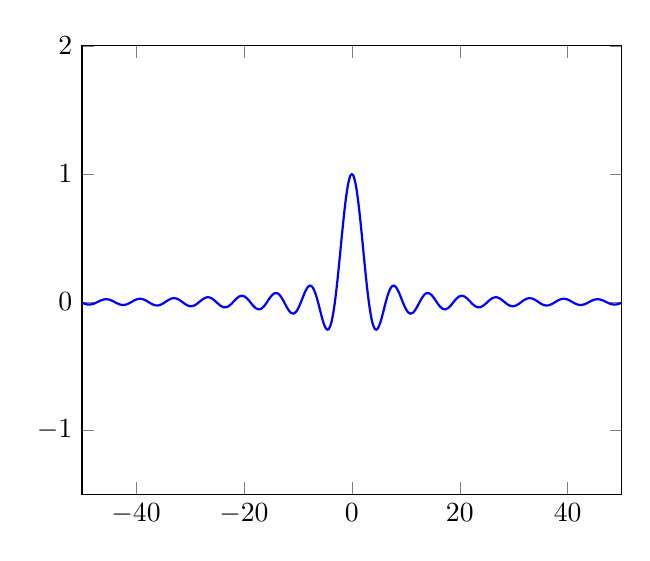
\begin{tikzpicture}
     
    \begin{axis}[
        xmin = -50, xmax = 50,
        ymin = -1.5, ymax = 2.0]
        \addplot[
            domain = -50:50,
            samples = 200,
            smooth,
            thick,
            blue,
        ] {sin(deg(x))) / x};
    \end{axis}
     
\end{tikzpicture}
    
\end{center}

\newpage

\section*{How do you sharpen an image?}

A sharpening filter is a type of filter that enhances the edges and details of an image. It works by amplifying the high-frequency components of the image, which corresponds to edges and fine details (rapid changes in their surrounding). \\

To obtain the sharper version of an image we can apply a technique called unsharp masking. These are the steps to follow:

\begin{itemize}
    \item apply a blurring filter to the original image to obtain the low frequency components;
    \item subtract the low frequency components from the original image to obtain the high frequency components;
    \item add the high frequency components back to the original image. This will create a sharper version.
\end{itemize}

It's important to note that this technique will also amplify noise, so it should be used with caution.

\newpage

\section*{Describe the Canny edge detector. What are the steps involved in edge detection using this detector?}

The Canny Edge Detector is a technique that resorts on the gradient of the image to detect edges. It consists of the following steps:

\begin{enumerate}[start=0]
    \item \textbf{Grayscale the image}.
    \item \textbf{Noise reduction}: resorting on the gradient, the pipeline is very susceptible to noise in the image, so the first step is to apply a Gaussian filter to blur it. We use the Gaussian over a Box filter for various reasons, first two among them are the fact that Box filter leaves ringing artifacts in the image and the fact that Gaussian filter better preserves the edges.
    \item \textbf{Gradient computation}: the smoothed image is then filtered with a Sobel kernel (first derivative) both in the horizontal direction ($\frac{\partial f}{\partial x} = S_x \otimes f$) and in the vertical direction ($\frac{\partial f}{\partial y} = S_y \otimes f$). 
    Once we have the image gradient 
    \begin{center}
        \begin{equation*}
            \nabla f = \left[ \frac{\partial f}{\partial x}, \frac{\partial f}{\partial y} \right]
        \end{equation*}
    \end{center}
    we can compute the orientation and magnitude of the gradient at each pixel:
        \begin{equation*}
        \theta = \tan^{-1}{\left( \frac{\partial f}{\partial x} / \frac{\partial f}{\partial y} \right)}
    \end{equation*}
    \begin{center}
        Direction
    \end{center}

    \begin{equation*}
        \|\nabla f\| = \sqrt{\left( \frac{\partial f}{\partial x} \right)^2 + \left( \frac{\partial f}{\partial y} \right)^2}
    \end{equation*}
    \begin{center}
        Intensity
    \end{center}
    \item \textbf{Non-maximum suppression}: ideally, the final image should have thin edges, thus we must perform non-maximum suppression to thin out the edges to a single pixel in width; the algorithm goes through all the points on the gradient intensity matrix and finds the pixels with the maximum value in the edge directions. The purpose of the algorithm is to check if the pixels on the same direction are more or less intense than the ones being processed. If the pixel (i, j) is being processed and the pixels on the same direction are (i, j-1) and (i, j+1), if one of those two pixels is more intense than the one being processed, then only the more intense one is kept.
    \item \textbf{Double threshold}: the double thresholding step is then applied to the resulting image with thin edges;
    it aims at identifying 3 kinds of pixels:
    \begin{itemize}
        \item \textbf{Strong pixels} are pixels that have an intensity so high that we are sure they contribute to the final edge;
        \item \textbf{Weak pixels} are pixels that have an intensity value that is not enough to be considered as strong ones, but yet not small enough to be considered as non-relevant for the edge detection;
        \item Other pixels are considered as \textbf{non-relevant} for the edge.
    \end{itemize}
    The threshold values are chosen empirically.
    \item \textbf{Linking}: based on the threshold results, the hysteresis consists of transforming weak pixels into strong ones if and only if at least one of the pixels around the one being processed is a strong one.
    
\end{enumerate}

Threshold and linking steps are also referred to as hysteresis.

\newpage

\section*{What is aliasing? How to deal with it?}
 
Images are a discrete, sampled representation of a continuous signal. If we want to sample a signal, it is possible to do it in such a way that the signal can later be reconstructed. The Nyquist sampling theorem states that the sample rate needs to be at least 2 times the highest frequency component (cutoff frequency) of the input signal to guarantee correct reconstruction. That rate is called Nyquist rate. If we don't respect this rate and we use a lower one, we have undersampling. If we undersample an image, like any other kind of signal, we won't be able to reconstruct it without information loss. On the other hand it is always possible to confuse a signal with one of higher frequency even if we sample correctly. \\

Reconstructing an image after undersampling generates an effect called aliasing. Aliasing occurs when the sampling rate or resolution is insufficient to accurately capture or represent the original signal. \\

Common ways to deal with aliasing are:

\begin{itemize}
    \item Oversampling the signal (sample with a rate over the Nyquist rate;
    \item Smooth the signal beforehand to remove some of the details that cause aliasing (high frequency components);
\end{itemize}

When we work with images we can mitigate aliasing by applying a smoothing filter (Gaussian, Box, ...) before the downsampling.

\newpage

\section*{What Gaussian Image Pyramids are? What are they used for? How they differ from Laplacian Image Pyramids?}

Image pyramids are a type of multi-scale representation of an image, where the original image is successively down-sampled to create a series of smaller versions each representing a different level of detail.
They are important for a variety of computer vision tasks:

\begin{itemize}
    \item Multi-scale image analysis: by using image pyramids we can process an image at different scales, allowing us to detect objects or features that may appear at different sizes in the image;
    \item Feature extraction: we can use image pyramids to extract features from different levels of the pyramid that capture different levels of detail;
    \item Image blending: image pyramids can be used for image blending, a task in which we want to seamlessly combine two images of different sizes and resolutions. 
\end{itemize}

The whole image pyramid is just 4/3 times the size of the original image.

A Gaussian Image Pyramid is obtained by repeatedly:
\begin{itemize}
    \item Applying a Gaussian filter to the image;
    \item Downsampling it
\end{itemize}

While a Gaussian image pyramid can provide useful information about the overall structure and coarse details of the image at different scales, it does not contain sufficient information to reconstruct the original image with high precision. The blurring and subsampling operations in the pyramid discard certain high-frequency details, resulting in a loss of information.

To reconstruct the original image from a Gaussian image pyramid, you would typically need to combine it with a corresponding Laplacian image pyramid. The Laplacian pyramid represents the difference between each level of the Gaussian pyramid and an upsampled version of the next level (smaller image). By combining the Gaussian and Laplacian pyramids, it is possible to reconstruct the original image with higher fidelity.

The steps to build a Laplacian Pyramid are the following:

\begin{itemize}
    \item Creating a Gaussian Image Pyramid. The Gaussian Pyramid is computed by repeatedly applying a Gaussian filter to the image and then downsampling it;
    \item Creating each level of the Laplacian Image Pyramid by subtracting from the corresponding layer of the Gaussian the upsampled version of the layer above it (smaller image).
\end{itemize}

\begin{equation*}
    L_k(I) = G_k(I) - u(G_{k+1}(I))
\end{equation*}

\begin{center}
    \textit{$I$ is the input image} \\
    \textit{$L_k(I)$ is the $k$-th level of the Laplacian pyramid} \\
    \textit{$G_k(I)$ is the $k$-th level of the Gaussian pyramid} \\
    \textit{$u(\cdot)$ is a 2x scale-up operation}
\end{center}

\newpage

\section*{Describe different kind of feature descriptors. In particular describe the Histogram of Oriented Gradients (HOG) applied to human detection.}

The term \textbf{local feature} refer to distinctive patterns or structures in an image that can be used to identify and describe specific regions of the image. Once the local features have been identified and extracted (feature extraction) from an image, they can be used to create a feature vector that describes the image (feature descriptor). This feature vector can be used for tasks such as object recognition or image matching, by comparing the features of different images and identifying those that are most similar. \\

A desirable feature descriptor should possess certain invariance properties to ensure robustness and generalization across different conditions. Here are some common types of invariance that feature descriptors aim to achieve:

\begin{itemize}
    \item \textbf{Scale invariance}: A feature descriptor should be able to detect and describe visual features regardless of their scale. This means that the descriptor should provide consistent representations even when the size of the object or the image changes.
    \item \textbf{Rotation invariance}: An effective feature descriptor should be able to recognize and describe features irrespective of their orientation or rotation in the image. This allows the descriptor to match features that are in different orientations or are subject to rotational transformations.
    \item \textbf{Affine invariance}: Affine transformations include not only rotations but also shearing, scaling, and translation. A desirable feature descriptor should be able to maintain consistency in the feature representation despite these types of transformations.    
    \item \textbf{Illumination invariance}: Lighting conditions can significantly affect the appearance of visual features. A good feature descriptor should be able to provide consistent representations regardless of changes in lighting, ensuring robustness to illumination variations.
\end{itemize}

We have various types of feature descriptors. Some naive options include:

\begin{itemize}
    \item \textbf{image gradients}: use the intensity variation between pixels in a window; this way the feature is invariant to absolute intensity changes; \textbf{How can it be less sensitive to deformations?}
    \item \textbf{color histogram}: count the colors in the window using a histogram; this is invariant to changes in scale and rotation; the problem with this approach is that \textbf{we loose spatial information}: two completely different patches with the same colors will have the same descriptor.
    \item \textbf{orientation normalization}: use the dominant image gradient direction to normalize the orientation of the patch; this is typically achieved by computing the dominant orientation of the image feature and then rotating the image patch; the problem with this approach is that orientation of an image feature can be sensitive to changes in scale, which can lead to inconsistencies in the descriptor when comparing features at different scales.
\end{itemize}

One of the most popular descriptors out there is the Histogram of Oriented Gradients (HOG) descriptor. The Histogram of Oriented Gradients (HOG) descriptor is a widely used feature extraction technique in computer vision. It is particularly effective for object detection and pedestrian recognition tasks. The main steps are:

\begin{itemize}
    \item \textbf{Preprocessing}: preprocess the image to bring down the width to height ratio to 1:2 for ease of computation;
    \item \textbf{Divide the image into $8 \times 8$ patches}. For each patch:
    \begin{itemize}
        \item \textbf{Computing image gradients} for each pixel in the $8 \times 8$ patch;
        \item \textbf{Compute magnitude and orientation} for each pixel in the $8 \times 8$ patch;
        \item \textbf{Generate an histogram} with magnitude and orientation; this results in a $1 \times 9$ vector describing the patch;
    \end{itemize}
    \item \textbf{Normalize the gradients}: we need to normalize the gradients by taking $16 \times 16$ blocks. Each block has 4 histograms which can be concatenated to form a $1 \times 36$ vector.
    This vector is normalized with L2 norm. It describes the feature that is at the centroid of the $16 \times 16$ block;
    \item Shift the $16 \times 16$ window by 8 pixels and go on. 
\end{itemize}

\newpage

\section*{List the main steps of the Harris corner detector.}

The Harris Corner Detector consists of the following steps. \\

For each pixel $(x, y)$:
\begin{enumerate}[start=0]
    \item \textbf{Preprocessing}: convert the original image I to grayscale;
    \item \textbf{Compute the derivatives $I_x$ and $I_y$ over a small region surrounding the pixel} by convolving it with a first derivative kernel, like the Sobel operator. We obtain $S_x$ and $S_y$. We can convolve the region with the derivative of a Gaussian to have better results instead.
    \item \textbf{Subtract the mean from each gradient} to eliminate the influence of the global intensity changes;
    \item \textbf{Compute the second moment matrix/covariance matrix over the window}: 
    \begin{center}
            \begin{equation*}
                M(x,y) = \sum_{(x,y) \in W}
                \begin{bmatrix}
                S_{x^2}(x,y) & S_{xy}(x,y) \\
                S_{xy}(x,y) & S_{y^2}(x,y)
                \end{bmatrix}
            \end{equation*}
    \end{center}
    The relationship between the covariance matrix and the second moment matrix is that the covariance matrix can be computed from the second moment matrix. The covariance matrix is essentially a normalized version of the second moment matrix. It is obtained by dividing each element of the second moment matrix by the number of pixels in the local neighborhood and subtracting the mean values. This normalization process accounts for the scale and makes the covariance matrix more suitable for statistical analysis.
    We will obtain a $4\times4$ matrix;
    \item \textbf{Compute eigenvalues and eigenvectors} of the second moment matrix;
    \item \textbf{Use threshold on eigenvalues to detect corners}:
    \begin{itemize}
        \item if $\lambda_1$ and $\lambda_2$ are small, then $|R|$ is small and the region is flat;
        \item if $\lambda_1 >> \lambda_2$ or $\lambda_1 <<\lambda_2$, then $|R| < 0$ and the region is an edge;
        \item if $\lambda_1 \approx \lambda_2$ and both eigenvalues are large, then $R$ is large and the region is a corner;
    \end{itemize}
    This classification derives from the Harris response for that pixel:
    \begin{center}
            \begin{equation*}
                R = det(M) - k\ tr(M)^2 = \lambda_1 \lambda_2 - k\ (\lambda_1 + \lambda_2)^2
            \end{equation*}
    \end{center}
    that as we can see depends on the eigenvalues for $M$.
\end{enumerate}

\newpage

\section*{Is the Harris corner detector robust with respect to uniform intensity changes in the image i.e. uniform intensity shifts and intensity scaling? Justify your answer. Is the Harris corner detector robust with respect to rotation? Justify your answer.} 

\textbf{Harris Corner Detector is invariant with respect to uniform intensity shifts in the image}: shifting the image uniformly does not affect the gradients of the image. The Harris Corner Detector operates on the gradients so any constant shift in intensity values will be cancelled out when computing the gradients. \\

\textbf{Harris Corner Detector is not invariant to intensity scale}: if the intensity scale of the image is changed, the gradients and the resulting structure tensor (second moment matrix) will also change. As a result, the corner response values (R) and the eigenvalues will be affected. In other words, if the intensity scale of the image is altered, the Harris Corner Detector's performance may be affected, and it may not accurately detect corners. \\

\textbf{Harris Corner Detector is invariant to rotation}: when an image is rotated, the local intensity variations around a corner point remain the same relative to the corner itself. Although the pixel position may change due to the rotation, the gradient of the image, which is what the Harris Corner Detector examines, remains unchanged. \\

\textbf{Harris Corner Detector is not invariant to scale}: in edge detection, the goal is to identify boundaries or transitions between regions of the image that have different pixel values or intensities. This is typically achieved by computing the gradient of the image, which represents the rate of change in pixel values or intensities in different directions. However, the gradient operator used in edge detection is typically based on a fixed kernel size or filter, such as the Sobel or Canny operators. This means that \textbf{the operator is tuned to detect edges at a specific scale or size of features in the image}. If the feature in the image are larger or smaller than the scale the operator is tuned to, the resulting edge or corner detection may not be accentuate or may miss important features.

\newpage

\section*{Why isn't a perceptron enough to model non linearly-separable data?}

A perceptron is a type of artificial neural network that is commonly used for classification problems. It takes a set of inputs, multiplies them by weights, adds up a bias term and then applies an activation function  to the result to produce an output. The perceptron algorithm adjusts the weights until the produced output matches the desired one. \\

If the data is linearly separable, meaning that there exists a line or a hyperplane that can separate the data points of different classes, then a single perceptron can learn this separation boundary. This is because the activation function of a perceptron is usually a step function, which produces a binary output based on the weighted sum of the inputs. Thus, if the data is linearly separable, the perceptron can learn the weights that define the separation boundary. \\

However, if the data is not linearly separable, then a single perceptron cannot accurately classify the data. In this case, more complex models such as multilayer perceptrons (MLPs) or support vector machines (SVMs) may be needed. \\

Another way could be to use a non-linear activation function to introduce non linearities into the (yet simple) network.

\newpage

\section*{What are the most common activation functions? Why are they important?}

Among all the activation functions, the most common are:

\begin{itemize}
    \item \textbf{Sigmoid}: the sigmoid function maps any input value to a value between $0$ and $1$. It is used in binary classification problems;

    \begin{equation*}
        \sigma(x) = \frac{1}{1 + e^{-x}}
    \end{equation*}
    
    \item \textbf{ReLU}: the ReLU maps any input value to $0$ if it is negative and to the same value if it is positive. It is used in deep neural networks due to its simplicity and ability to prevent vanishing gradients;

    \begin{equation*}
        f(x) = max(0, x)
    \end{equation*}
    
    \item \textbf{Tanh}: the tanh function maps any input to a value between $-1$ and $1$. It is used in some neural networks, particularly those with a smaller number of layers;

    \begin{equation*}
        f(x) = \frac{e^{x}-e^{-x}}{e^{x}+e^{-x}}            
    \end{equation*}
    
    \item \textbf{Softmax}: the softmax function maps a vector of values to a probability distribution. It is commonly used in the output layer of a neural network for multi-class classification problems.

    \begin{equation*}
        f(x_i) = \frac{e^{x_i}}{\sum_{j=1}^{K}e^{x_j}}
    \end{equation*}
    
\end{itemize}

Activation functions are important because they introduce non-linearity to the neural network, allowing it to model more complex relationships between inputs and outputs. Non-linear activation functions enable neural networks to learn more complex decision boundaries and make the network more expressive.

\newpage 

\section*{What is the difference between error function, cost function and loss function?}

In machine learning the terms error function, cost function and loss function are often used interchangeably. However, there are some subtle differences between them:

\begin{itemize}
    \item \textbf{Error function}: an error function is a mathematical object that measures the difference between two terms;
    \item \textbf{Cost function}: a cost function is similar to an error function but it is often used in optimization problems, where we don't have a target value a priori; we use a cost function to find the set of parameters that results in the lowest possible cost;
    \item \textbf{Loss function}: a loss function is used to measure the difference between a predicted output and the actual one in a machine learning problem. 
\end{itemize}

The loss function is used to compute the error for a single training example, the overall cost function is computed as the average of the loss function over all the training examples.

\newpage

\section*{What are the most common loss functions? What are they used for?}

A loss function is a mathematical function that measures the difference between the predicted output of a model and the true output (i.e., the target) for a given input. The goal of the model is to minimize this difference during training, by adjusting the model's parameters (i.e., weights and biases). 

\begin{equation*}
    L(f(x^{(i)};W), y^{(i)})
\end{equation*}

The most common loss functions include:
\begin{itemize}
    \item \textbf{Mean Squared Error (MSE)}: MSE is a common loss function used for \textbf{regression problems} (problem that involve finding a function that maps input variables to a continuous output variable, which can then be used to make predictions on new or unseen data). It measures the average squared difference between the predicted and true values.

    \begin{equation*}
        MSE = \frac{1}{N} \sum_{i=1}^{N}(y_i - \hat{y_i})^2
    \end{equation*}

    \item \textbf{Binary Cross-Entropy (BCE)}: BCE is a common loss function used for \textbf{binary classification problems}. It measures the difference between the predicted and true class labels.

    \begin{equation*}
        BCE = -\frac{1}{N} \sum_{i=1}^{N} y_i log(\hat{y_i}) + (1-y_i)log(1-\hat{y_i})
    \end{equation*}

    \item \textbf{Categorical Cross-Entropy (CCE):} CCE is a common loss function used for multi-class classification problems. It measures the difference between the predicted and true class probabilities.

    \begin{equation*}
        CCE = -\frac{1}{N} \sum_{i=1}^{N}\sum_{j=1}^{K}y_{ij} log(\hat{y_{ij}})
    \end{equation*}

    \item \textbf{Kullback-Leibler (KL) Divergence}: KL divergence is a measure of the difference between two probability distributions. It is often used as a loss function for generative models, such as variational autoencoders.

    \begin{equation*}
        KL(p|q) = \sum_{i}p(i)log\frac{p(i)}{q(i)}
    \end{equation*}
    
\end{itemize}

\newpage

\section*{Talk about the problems of vanishing and exploding gradients in neural networks and how can we overcome them.}

Vanishing and exploding gradients are common problems that can occur in deep neural networks during training.

Vanishing gradients occur when the gradients calculated in the backpropagation step of training become very small as they are propagated backwards through the network. This means that the weights in the early layers of the network are updated very slowly, or not at all, resulting in a slow or stalled learning process. This problem is particularly common in deep networks with many layers, as the gradients can become exponentially smaller as they propagate backwards through the layers.

On the other hand, exploding gradients occur when the gradients calculated in the backpropagation step become very large as they are propagated backwards through the network. This can result in weights being updated too aggressively, leading to unstable and erratic training.

To overcome these problems, several techniques have been proposed, including:

\begin{itemize}
    \item \textbf{Weight initialization}: Setting appropriate initial weights for the network can help avoid the vanishing and exploding gradient problem. One popular method is to initialize the weights using a Gaussian distribution with a mean of zero and a standard deviation that depends on the number of input and output units.
    \item \textbf{Non-saturating activation functions}: Choosing activation functions that do not saturate (i.e., do not become flat) in the regions where the gradients are small can help alleviate the vanishing gradient problem. ReLU and its variants are good examples of non-saturating activation functions.
    \item \textbf{Gradient clipping}: Gradient clipping involves setting a threshold on the gradients during training, so that they do not exceed a certain value. This can help prevent the exploding gradient problem.
    \item \textbf{Batch normalization}: Batch normalization is a technique that normalizes the input to each layer in the network, reducing the internal covariate shift and helping to stabilize the gradients.
    \item \textbf{Residual connections}: Residual connections involve skipping one or more layers in a network, allowing the gradients to flow directly from one layer to another, which can help alleviate the vanishing gradient problem in very deep networks.
\end{itemize}

These techniques are widely used in modern deep learning frameworks and can help improve the stability and performance of neural networks during training.

\newpage

\section*{What is batch normalization and how can it be used to avoid the vanishing gradient problem?}

Batch normalization is a technique used in deep learning to standardize the inputs of each layer in a neural network so that the data is on a known, standard, scale. Why do we care to do that? \\

If we don't normalize the data \textbf{before passing it to the first layer} we may end up having in the dataset data points that are very high while others are very low. The larger datapoints in this non-normalized dataset can cause instability in neural networks because the relatively large inputs can cascade down through the layers of the network and cause imbalanced gradients, which may, in turn, cause the exploding gradient problem. The same thing for very low datapoints. \\

When we put all the inputs on the same scale we don't have such variance between datapoints anymore.

There is another problem that can arise even with normalized data: what if one of the weights becomes drastically larger than the other weights? This large weight will then cause the output from its corresponding neuron to be extremely large and this imbalance will again continue to cascade through the neural network causing instability. \textbf{This is why normalization is usually done at each layer}: we now talk about \textbf{batch normalization}. Everything we just mentioned about the batch normalization process occurs on a per batch basis.

Consider a batch of activations at some layer. To make each dimension zero-mean unit-variance apply:

\begin{equation*}
    \hat{x^{(k)}} = \frac{x^{(k)} - E[x^{(k)}]}{\sqrt{Var[x^{(k)}]}} 
\end{equation*}

\newpage

\section*{What are mini-batches and how can they lead to fast training?}

There are several ways to train a neural network:

\begin{itemize}
    \item \textbf{Batch Gradient Descent}: the batch size is equal to the size of the training set;
    \item \textbf{Stochastic Gradient Descent}: the batch size is equal to 1;
    \item \textbf{Mini-batch Gradient Descent}: the batch size is $1 < \text{batch size} < \text{size of the training set}$ 
\end{itemize}

Gradient Descent is an optimization algorithm used to train machine learning algorithms, most notably artificial neural networks used in deep learning. The job of the algorithm is to find a set of internal model parameters that perform well against some performance measure such as logarithmic loss or mean squared error. The algorithm relies on the backpropagation algorithm, which computes the contribution on the error of each parameter. \\

In neural networks, mini-batches refer to a subset of the training data that is used to update the model's parameters (weights and biases) during each iteration of the training process. \\

Training a neural network on a large dataset can be computationally expensive and memory-intensive. To mitigate these issues, the data is divided into smaller subsets called mini-batches. Each mini-batch contains a fixed number of examples, typically ranging from 16 to 512. During training, the model is trained on each mini-batch sequentially, and the parameters are updated based on the average loss across the examples in the mini-batch.

Using mini-batches has several advantages. First, it reduces the memory requirements of the training process, allowing the model to train on larger datasets than would otherwise be possible. Second, it allows for more frequent updates of the model's parameters, which can accelerate the convergence of the optimization process. Third, it can improve the generalization performance of the model by introducing randomness and reducing overfitting.

\newpage

\section*{What is overfitting? How can we overcome it?}

Overfitting is when a model is trained too well on the training data, to the point that it begins to memorize the training data rather than learning the underlying patterns or relationships among datapoitns. As a result, the model performs very well on the training data but poorly on new, unseen data. \\

Overfitting can occur when a model is too complex relative to the amount of training data available. This can happen when a model has too many parameters or when the model is trained for too long, allowing it to memorize the noise in the training data. \\

To overcome overfitting, there are several techniques that can be used:

\begin{itemize}
    \item \textbf{Cross-validation}: Cross-validation involves dividing the training data into multiple folds and using each fold as a validation set while training the model on the remaining folds. This helps to prevent overfitting by providing a more accurate estimate of the model's performance on new, unseen data. \\ 
    
    The main difference between cross-validation and k-fold cross-validation is that cross-validation typically involves splitting the data into two parts, a training set and a validation set, while k-fold cross-validation involves dividing the data into k parts and using each part as the validation set in turn.
    
    \item \textbf{Regularization}: Regularization techniques, such as L1 and L2 regularization, add a penalty term to the loss function during training, which discourages the model from overfitting by reducing the magnitude of the weights.
    
    \item \textbf{Dropout}: randomly drop out some of the neurons during training.
    
    \item \textbf{Early stopping}: Early stopping is a technique used to prevent overfitting by monitoring the loss on the validation set during training and stopping the training process when the validation error starts to increase.
    
    \item \textbf{Data augmentation}: Data augmentation involves creating new training data by applying transformations to the existing training data. This can help to increase the amount of training data and prevent overfitting. When we are dealing with images, data augmentation can be done with transformations on the image, cropping, cutout, color jitter, mixup and so on.
\end{itemize}

\newpage

\section*{Why does adding a regularization term to the loss function helps reducing overfitting?}

To implement regularization we simply add a term to the loss function that penalizes for large weights. 

\begin{itemize}
    \item with L2 regularization we add the sum of the square norms of the weight matrices multiplied by a small constant to the loss function;
    \begin{equation*}
        \hat{loss} = loss + x        
    \end{equation*}
    \begin{equation*}
        x = \frac{\lambda}{2m}\sum_{j=1}^n |w_j|^2
    \end{equation*}
    A regression model that implement L2 regularization is also called \textbf{Ridge regression}.
    \item with L1 regularization we add the absolute value of magnitude of the weight matrices as penalty term to the loss function.
    \begin{equation*}
        \hat{loss} = loss + x        
    \end{equation*}
    \begin{equation*}
        x = \lambda \sum_{j=1}^p |w_j|
    \end{equation*}
    
    A regression model that implement L1 regularization is also called \textbf{Lasso regression}.
\end{itemize}

$\lambda$ is called \textbf{regularization parameter} and is another hyperparameter that we can tune.\\

Adding a regularization term to the loss function helps reduce overfitting by imposing a penalty on the model for having large weights. By adding a regularization term to the loss function, the model is encouraged to find a solution that is both accurate on the training data and simple enough to generalize well to new data. This helps to prevent overfitting by reducing the model's complexity and improving its ability to generalize.

\newpage

\section*{What is transfer learning?}

Transfer learning is a machine learning technique that involves taking knowledge learned from one task and applying it to another task. The idea is to transfer the knowledge gained from solving one problem to help solve a different, but related problem.

In traditional machine learning, each task is typically trained from scratch using a separate set of data. However, in transfer learning, a pre-trained model is used as a starting point for a new task. The pre-trained model has already learned some useful features or patterns from a different but related task, and these features can be re-used to speed up the training process and improve the performance of the model on the new task.

For example, a pre-trained model that was trained to recognize objects in images could be fine-tuned for a new task, such as recognizing faces in images. \textbf{The lower layers of the pre-trained model, which learn general features such as edges and corners, can be kept fixed, while the upper layers, which are task-specific, can be modified to learn the new task.}

Transfer learning has several advantages over training a model from scratch. It can reduce the amount of data and computational resources required to train a new model, and it can improve the performance of the model on the new task by leveraging the knowledge gained from solving related tasks.

\end{document}
